\makeatletter
\newcommand{\diagdenomb}{\@ifstar{\@diagdenomb}{\@@diagdenomb}}
\newcommand{\@diagdenomb}{\begin{figure}[htbp]
    \centering
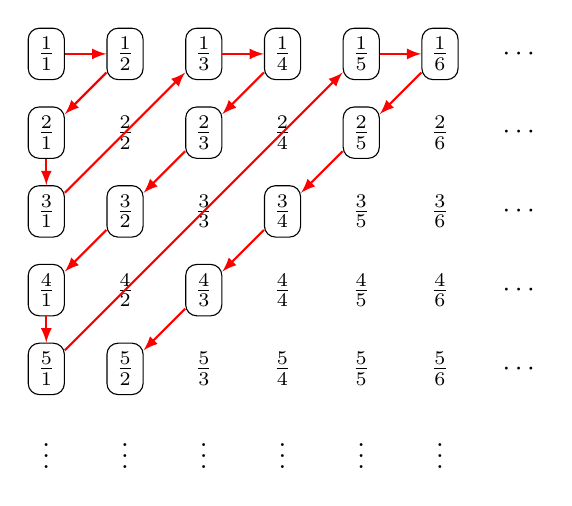
\begin{tikzpicture}
\tikzstyle{keepstyle} =[rectangle, rounded corners, draw, fill=white]
\node at (0,0) {$\vdots$};
\node[keepstyle] (51) at (0,1) {$\frac{5}{1}$};
\node[keepstyle] (41) at (0,2) {$\frac{4}{1}$};
\node[keepstyle] (31) at (0,3) {$\frac{3}{1}$};
\node[keepstyle] (21) at (0,4) {$\frac{2}{1}$};
\node[keepstyle] (11) at (0,5) {$\frac{1}{1}$};
\node at (1,0) {$\vdots$};
\node[keepstyle] (52) at (1,1) {$\frac{5}{2}$};
\node at (1,2) {$\frac{4}{2}$};
\node[keepstyle] (32) at (1,3) {$\frac{3}{2}$};
\node at (1,4) {$\frac{2}{2}$};
\node[keepstyle] (12) at (1,5) {$\frac{1}{2}$};
\node at (2,0) {$\vdots$};
\node at (2,1) {$\frac{5}{3}$};
\node[keepstyle] (43) at (2,2) {$\frac{4}{3}$};
\node at (2,3) {$\frac{3}{3}$};
\node[keepstyle] (23) at (2,4) {$\frac{2}{3}$};
\node[keepstyle] (13) at (2,5) {$\frac{1}{3}$};
\node at (3,0) {$\vdots$};
\node at (3,1) {$\frac{5}{4}$};
\node at (3,2) {$\frac{4}{4}$};
\node[keepstyle] (34) at (3,3) {$\frac{3}{4}$};
\node at (3,4) {$\frac{2}{4}$};
\node[keepstyle] (14) at (3,5) {$\frac{1}{4}$};
\node at (4,0) {$\vdots$};
\node  at (4,1) {$\frac{5}{5}$};
\node at (4,2) {$\frac{4}{5}$};
\node at (4,3) {$\frac{3}{5}$};
\node[keepstyle] (25) at (4,4) {$\frac{2}{5}$};
\node[keepstyle] (15) at (4,5) {$\frac{1}{5}$};
\node at (5,0) {$\vdots$};
\node  at (5,1) {$\frac{5}{6}$};
\node at (5,2) {$\frac{4}{6}$};
\node at (5,3) {$\frac{3}{6}$};
\node at (5,4) {$\frac{2}{6}$};
\node[keepstyle] (16) at (5,5) {$\frac{1}{6}$};
\node at (6,1) {$\cdots$};
\node at (6,2) {$\cdots$};
\node at (6,3) {$\cdots$};
\node at (6,4) {$\cdots$};
\node at (6,5) {$\cdots$};
\draw [-latex,red, thick] (11) -- (12);
\draw [-latex, red, thick] (12) -- (21);
\draw [-latex, red, thick] (21) -- (31);
\draw [-latex, red, thick] (31) -- (13);
\draw [-latex, red, thick] (13) -- (14);
\draw [-latex, red, thick] (14) -- (23);
\draw [-latex, red, thick] (23) -- (32);
\draw [-latex, red, thick] (32) -- (41);    
\draw [-latex, red, thick] (41) -- (51);
\draw [-latex, red, thick] (51) -- (15);
\draw [-latex, red, thick] (15) -- (16);
\draw [-latex, red, thick] (16) -- (25);
\draw [-latex, red, thick] (25) -- (34);
\draw [-latex, red, thick] (34) -- (43);
\draw [-latex, red, thick] (43) -- (52);
\end{tikzpicture}
%\caption*{Dénombrabilité de $\mathbb{Q}$}
\end{figure}
}
\newcommand{\@@diagdenomb}{\begin{figure}[htbp]
    \centering
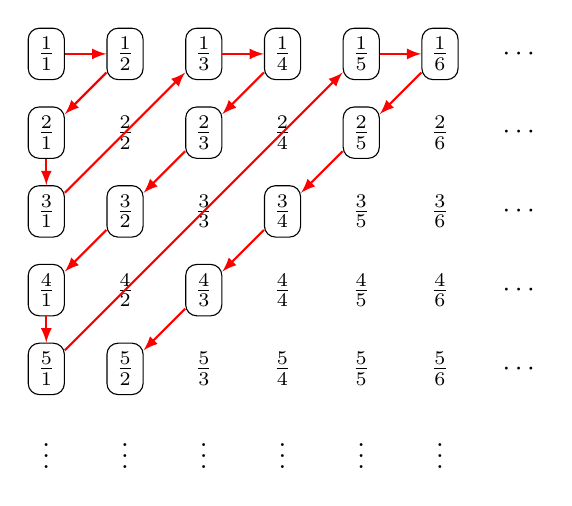
\begin{tikzpicture}
\tikzstyle{keepstyle} =[rectangle, rounded corners, draw, fill=white]
\node at (0,0) {$\vdots$};
\node[keepstyle] (51) at (0,1) {$\frac{5}{1}$};
\node[keepstyle] (41) at (0,2) {$\frac{4}{1}$};
\node[keepstyle] (31) at (0,3) {$\frac{3}{1}$};
\node[keepstyle] (21) at (0,4) {$\frac{2}{1}$};
\node[keepstyle] (11) at (0,5) {$\frac{1}{1}$};
\node at (1,0) {$\vdots$};
\node[keepstyle] (52) at (1,1) {$\frac{5}{2}$};
\node at (1,2) {$\frac{4}{2}$};
\node[keepstyle] (32) at (1,3) {$\frac{3}{2}$};
\node at (1,4) {$\frac{2}{2}$};
\node[keepstyle] (12) at (1,5) {$\frac{1}{2}$};
\node at (2,0) {$\vdots$};
\node at (2,1) {$\frac{5}{3}$};
\node[keepstyle] (43) at (2,2) {$\frac{4}{3}$};
\node at (2,3) {$\frac{3}{3}$};
\node[keepstyle] (23) at (2,4) {$\frac{2}{3}$};
\node[keepstyle] (13) at (2,5) {$\frac{1}{3}$};
\node at (3,0) {$\vdots$};
\node at (3,1) {$\frac{5}{4}$};
\node at (3,2) {$\frac{4}{4}$};
\node[keepstyle] (34) at (3,3) {$\frac{3}{4}$};
\node at (3,4) {$\frac{2}{4}$};
\node[keepstyle] (14) at (3,5) {$\frac{1}{4}$};
\node at (4,0) {$\vdots$};
\node  at (4,1) {$\frac{5}{5}$};
\node at (4,2) {$\frac{4}{5}$};
\node at (4,3) {$\frac{3}{5}$};
\node[keepstyle] (25) at (4,4) {$\frac{2}{5}$};
\node[keepstyle] (15) at (4,5) {$\frac{1}{5}$};
\node at (5,0) {$\vdots$};
\node  at (5,1) {$\frac{5}{6}$};
\node at (5,2) {$\frac{4}{6}$};
\node at (5,3) {$\frac{3}{6}$};
\node at (5,4) {$\frac{2}{6}$};
\node[keepstyle] (16) at (5,5) {$\frac{1}{6}$};
\node at (6,1) {$\cdots$};
\node at (6,2) {$\cdots$};
\node at (6,3) {$\cdots$};
\node at (6,4) {$\cdots$};
\node at (6,5) {$\cdots$};
\draw [-latex,red, thick] (11) -- (12);
\draw [-latex, red, thick] (12) -- (21);
\draw [-latex, red, thick] (21) -- (31);
\draw [-latex, red, thick] (31) -- (13);
\draw [-latex, red, thick] (13) -- (14);
\draw [-latex, red, thick] (14) -- (23);
\draw [-latex, red, thick] (23) -- (32);
\draw [-latex, red, thick] (32) -- (41);    
\draw [-latex, red, thick] (41) -- (51);
\draw [-latex, red, thick] (51) -- (15);
\draw [-latex, red, thick] (15) -- (16);
\draw [-latex, red, thick] (16) -- (25);
\draw [-latex, red, thick] (25) -- (34);
\draw [-latex, red, thick] (34) -- (43);
\draw [-latex, red, thick] (43) -- (52);
\end{tikzpicture}
\caption{Dénombrabilité de $\mathbb{Q}$}
    \label{fig:denombQ}
\end{figure}
}
\makeatother
\graphicspath{{./figures/}} % pour les images, plus besoin d'écrire "./figures"
\newcommand{\diagbij}{\begin{figure}[htbp]
	\centering
	\begin{tikzpicture}[ele/.style={fill=black,circle,minimum width=.8pt,inner sep=1pt},every fit/.style={ellipse,draw,inner sep=-2pt}]
	\node[ele,label=left:$a$] (a1) at (0,4) {};    
	\node[ele,label=left:$b$] (a2) at (0,3) {};    
	\node[ele,label=left:$c$] (a3) at (0,2) {};
	\node[ele,label=left:$d$] (a4) at (0,1) {};
	\node[ele,label=left:$d$] (a5) at (0,1) {};
	\node[ele,fill=roug,label=right:$1$] (b1) at (4,4) {};
	\node[ele,fill=roug,label=right:$2$] (b2) at (4,3) {};
	\node[ele,fill=roug,label=right:$3$] (b3) at (4,2) {};
	\node[ele,fill=roug,label=right:$4$] (b4) at (4,1) {};
	
	\node[fill=bleu,draw=bleu,fill opacity=0.3,fit= (a1) (a2) (a3) (a4) (a5),minimum width=2cm] {} ;
	\node[fill=roug,draw=roug,fill opacity=0.3,fit= (b1) (b2) (b3) (b4),minimum width=2cm] {} ;  
	\draw[->,thick,shorten <=2pt,shorten >=2] (a1) -- (b4);
	\draw[->,thick,shorten <=2pt,shorten >=2] (a2) -- (b2);
	\draw[->,thick,shorten <=2pt,shorten >=2] (a3) -- (b1);
	\draw[->,thick,shorten <=2pt,shorten >=2] (a4) -- (b3);
	\end{tikzpicture}
	\caption{diagramme d'une fonction bjective}
	\label{fig-fonctbij}
\end{figure}}

\newcommand{\compfonc}{
\begin{figure}
    \centering
    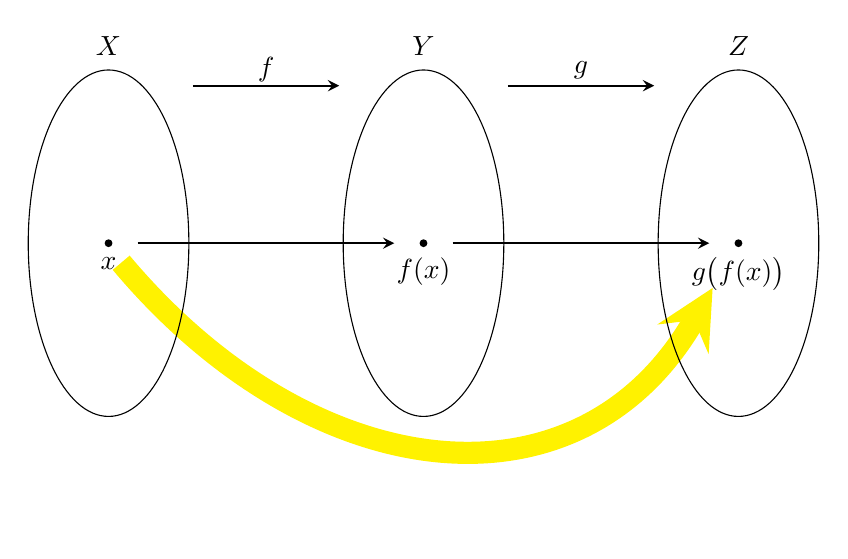
\begin{tikzpicture}[
    >=stealth,
    bullet/.style={
        fill=black,
        circle,
        minimum width=1pt,
        inner sep=1pt
    },
    projection/.style={
        ->,
        thick,
        shorten <=2pt,
        shorten >=2pt
    },
    every fit/.style={
        ellipse,
        draw,
        inner sep=0pt
    }
    ]
    \node at (2,4.7) {$f$};
    \draw[projection] (1,4.5) -- (3,4.5);
    \node at (0,5) {$X$};
    \node[bullet,label=below:$x$] (START)   at (0,2.5){};
    \node at (4,5) {$Y$};
    \node[bullet,label=below:$f(x)$] at (4,2.5){};
    \node at (6,4.7) {$g$};
    \draw[projection] (5,4.5) -- (7,4.5);
    \node at (8,5) {$Z$};
    \node[bullet,label=below:$g\big(f(x)\big)$] (END) at (8,2.5){};
    
    \draw [line width=8pt, yellow, shorten <=0.25cm,, shorten >=0.6cm, ->] (START.south) to[out=-50, in=-120, distance=4cm, ] (END);

    \draw (0,2.5) ellipse (1.02cm and 2.2cm);
    \draw (4,2.5) ellipse (1.02cm and 2.2cm);
    \draw (8,2.5) ellipse (1.02cm and 2.2cm);

    \draw[projection] (0.3,2.5) -- (3.7,2.5);
    \draw[projection] (4.3,2.5) -- (7.7,2.5);
    \end{tikzpicture}
    \caption{Caption}
    \label{fig:my_label}
\end{figure}}